\documentclass[%
    reprint,
    onecolumn,
    nofootinbib,
    amsmath,
    amssymb,
    aps,
    prstab,
]{revtex4-2}

\usepackage{graphicx} 
\usepackage{subcaption}

\begin{document}


\title{Supplementary Material for ``N-dimensional maximum-entropy tomography via particle sampling''}


\maketitle


\section{Comparison to GPSR}

%
\begin{figure}[b]
    \centering
    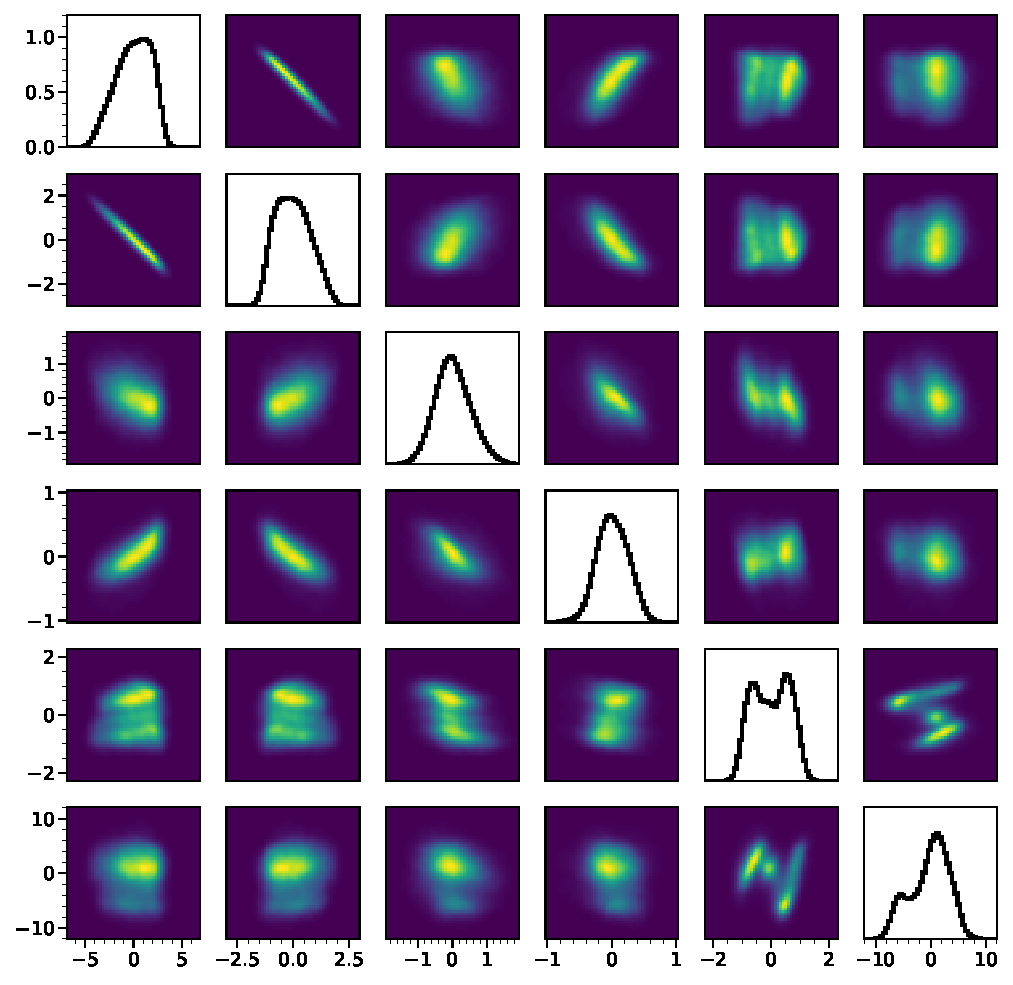
\includegraphics[width=0.66\linewidth]{fig_ment_corner_samp.pdf}
    \caption{Distribution of $9 \times 10^4$ particles sampled from the MENT reconstruction. A Gaussian filter with $\sigma = 1$ is applied to the histograms.}
\end{figure}
%

%
\begin{figure}[b]
    \centering
    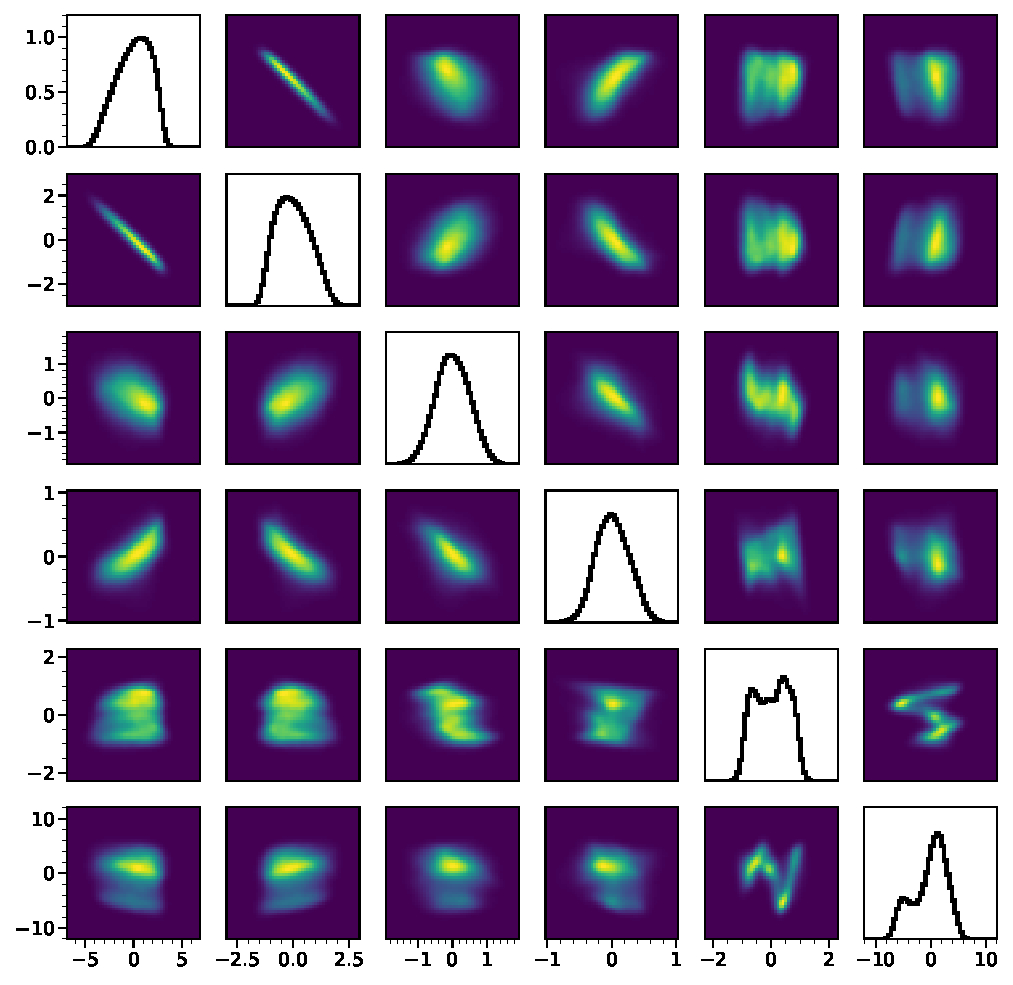
\includegraphics[width=0.66\linewidth]{fig_gpsr_corner_samp.pdf}
    \caption{Distribution of $9 \times 10^4$ particles sampled from the GPSR reconstruction. A Gaussian filter with $\sigma = 1$ is applied to the histograms.}
\end{figure}
%

%
\begin{figure}
    \centering
    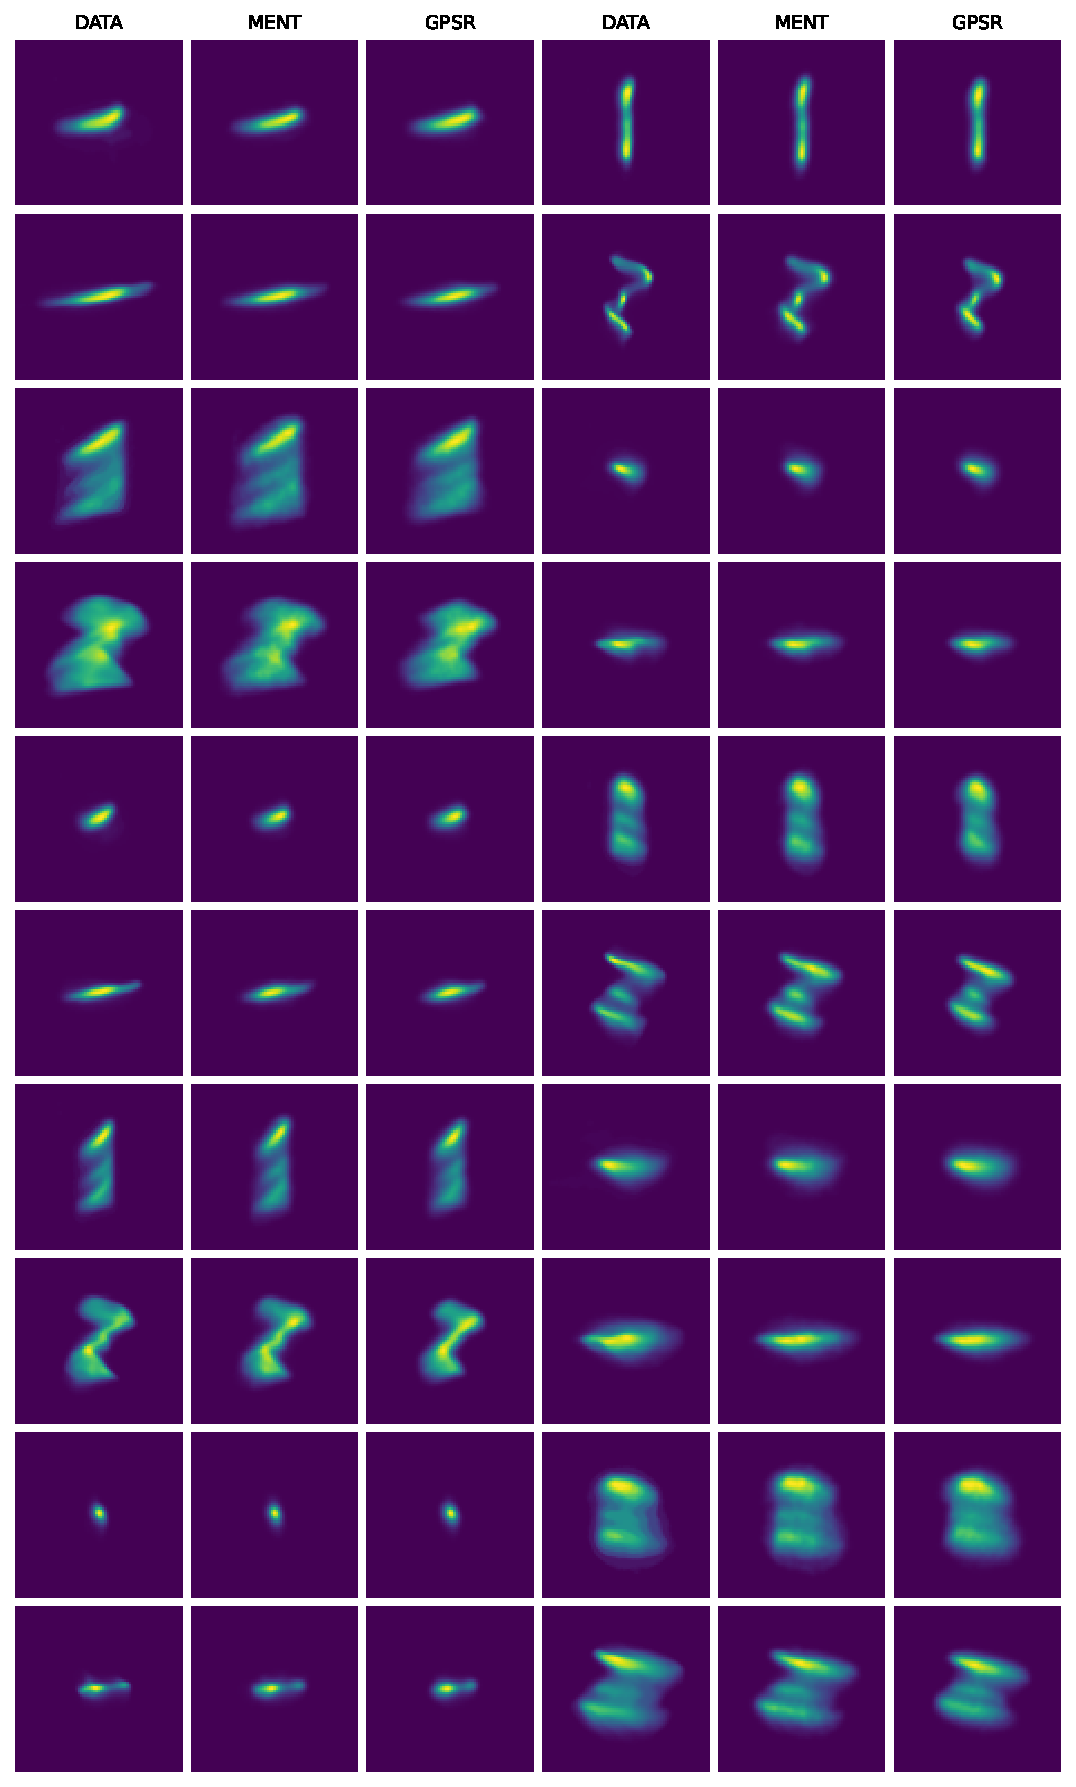
\includegraphics[width=0.66\linewidth]{fig_compare_data_train.pdf}
    \caption{Measured and predicted images from the training data set. Predictions are made from $9 \times 10^4$ particles sampled from each model (MENT/GPSR). A Gaussian filter with $\sigma = 1$ is applied to the predicted histograms. The images is split into two groups of three columns to fit on the page.}
    \label{fig:data-train}
\end{figure}
%

%
\begin{figure}
    \centering
    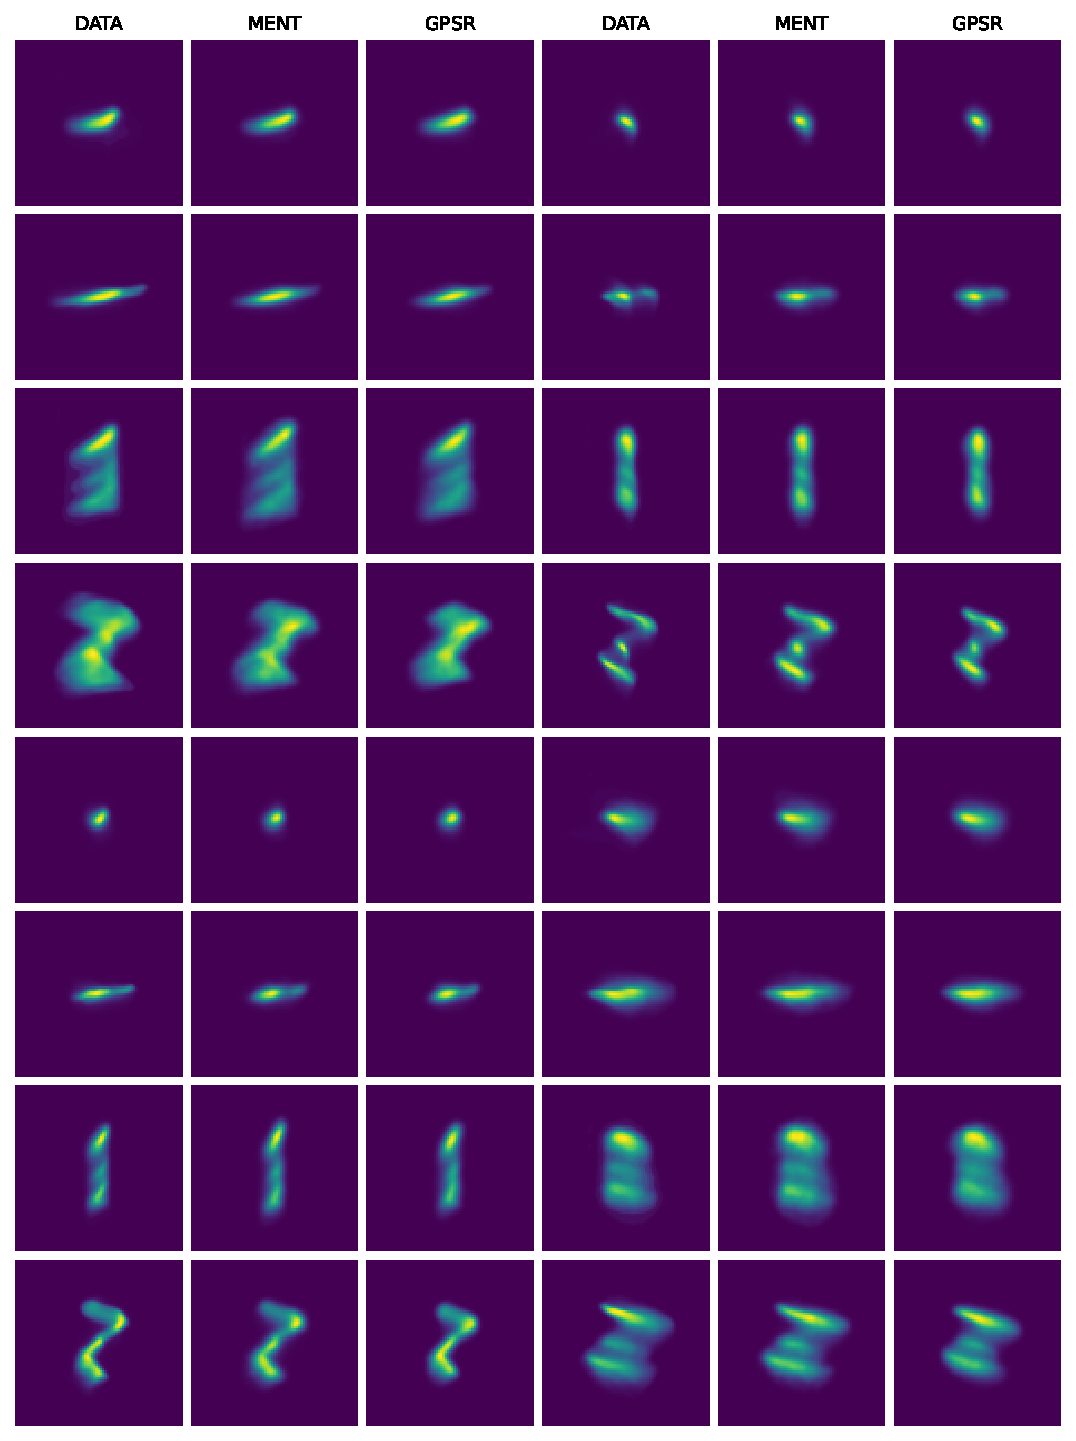
\includegraphics[width=0.66\linewidth]{fig_compare_data_test.pdf}
    \caption{Measured and predicted images from the testing data set. Predictions are made from $9 \times 10^4$ particles sampled from each model (MENT/GPSR). A Gaussian filter with $\sigma = 1$ is applied to the predicted histograms. The images is split into two groups of three columns to fit on the page.}
    \label{fig:data-train}
\end{figure}
%

\end{document}